\documentclass[12pt,a4paper]{article}
%-------------------------------------------
%---Packages--------------------------------
%-------------------------------------------
\usepackage[utf8]{inputenc}
%\usepackage[T1]{fontenc}
%\usepackage{txfonts}
\usepackage{amsmath}
\usepackage{amsthm}
\usepackage{amsfonts}
\usepackage{array}
\usepackage{amssymb}
\usepackage{blindtext}
\usepackage{caption}
\usepackage{color}
\usepackage{csquotes}	    %
\usepackage{enumitem}	    %pour mieux bosser avec les listes. ajoute option label
\usepackage[yyyymmdd]{datetime}        %pour définir date custom
\usepackage{etaremune}
\usepackage{environ}
\usepackage{fancybox}
\usepackage{fancyhdr} 	    % Custom headers and footers
\usepackage{fancyref}
%\usepackage{float}
\usepackage{floatrow}       %float and floatrow can't be together...
\usepackage{gensymb}
\usepackage{graphicx}
\usepackage[colorlinks=true, linkcolor=purple, citecolor=cyan]{hyperref}
\usepackage{footnotebackref}
\usepackage{lipsum}
\usepackage{mathtools}
\usepackage{multicol}	    %gérer plusieurs colonnes
\usepackage{setspace}
\usepackage{subcaption}
\usepackage{todonotes}	    %Bonne gestion des TODOs
%TODO commenté pour tester l'utilité... à voir% \usepackage[tc]{titlepic}      %Permet de mettre une image en page de garde
\usepackage{tikz}	    % Pour outil de dessin puissant
\usepackage{ulem}	    %underline sur plusieurs lignes (avec \uline{})
\usepackage{vmargin} 	    %gestion des marges, avec dans l'ordre : gauche, haut, droit, bas, en-tête, entre en-tête et texte, bas de page, hauteur entre bas de page et texte
\usepackage{wrapfig}
\usepackage{xcolor}
\usepackage{xparse}                    %Pour utiliser NewDocumentCommand et des arguments 'mmooo'
%\usepackage{fullpage} 	    %supprime toutes les marges allouées aux notes, aussi en haut et en bas

%\ExplSyntaxOn
\pagestyle{fancyplain}	    %Makes all pages in the document conform to the custom headers and footers

%-------------------------------------------
%---Document Commands-----------------------
%---------------------------{----------------
\NewDocumentCommand{\framecolorbox}{oommm}
 {% #1 = width (optional)
  % #2 = inner alignment (optional)
  % #3 = frame color
  % #4 = background color
  % #5 = text
  \IfValueTF{#1}%
   {\IfValueTF{#2}%
    {\fcolorbox{#3}{#4}{\makebox[#1][#2]{#5}}}%
    {\fcolorbox{#3}{#4}{\makebox[#1]{#5}}}%
   }%
   {\fcolorbox{#3}{#4}{#5}}%
 }%
%------------------------------------------------
%------------------ENGLISH----------------------
%----------------------------------------------

\NewDocumentCommand{\epflTitle}{mO{Olivier Cloux}O{\today}O{Notes de Cours en}D<>{../../Common}}%Arguments : Matière, Auteur, Date, Titre du doc
{
\begin{titlepage}
    \vspace*{\fill}
    \begin{center}
        \normalfont \normalsize
        \textsc{Ecole Polytechnique Fédérale de Lausanne} \\ [25pt] % Your university, school and/or department name(s)
        \textsc{#4} %Titre du doc
        \\ [0.4 pt]
        \horrule{0.5pt} \\[0.4cm] % Thin top horizontal rule
        \huge #1 \\ % Matière
        \horrule{2pt} \\[0.5cm] % Thick bottom horizontal rule
        
\includegraphics[width=8cm]{#5/EPFL_logo}
        ~\\[0.5 cm]
        \small\textsc{#2}\\[0.4cm]
        \small\textsc{#3}\\
        ~\\
        ~\\
        
\includegraphics[scale=0.5]{#5/creativeCommons}
    \end{center}
    \vspace*{\fill}
\end{titlepage}
}


%-------------------------------------------
%-------------MATH NEW COMMANDS-------------
%-------------------------------------------
\newcommand{\somme}[2]{\ensuremath{\sum\limits_{#2}^{#1}}}
\newcommand{\produit}[2]{\ensuremath{\prod\limits_{#2}^{#1}}}
\newcommand{\limite}{\lim\limits_}
\newcommand{\llimite}[3]{\limite{\substack{#1 \\ #2}}\left(#3\right)}	%limites à deux condiitons
\newcommand{\et}{\mbox{ et }}
\newcommand{\deriv}[1]{\ensuremath{\, \mathrm d #1}}	%sigle dx, dt,dy... des dérivées/intégrales
%\newcommand{\fx}{\ensuremath{f'(\textbf{x}_0 + h}}
\newcommand{\ninf}{\ensuremath{n \to \infty}}	       %pour les limites : n tend vers l'infini
\newcommand{\xinf}{\ensuremath{x \to \infty}}	       %pour les limites : x tend vers l'infini
\newcommand{\infint}{\ensuremath{\int_{-\infty}^{\infty}}}
\newcommand{\xo}{\ensuremath{x \to 0}}									%x to 0
\newcommand{\no}{\ensuremath{n \to 0}}									%n zéro
\newcommand{\xx}{\ensuremath{x \to x}}									%x to x
\newcommand{\Xo}{\ensuremath{x_0}}										%x zéro
\newcommand{\X}{\ensuremath{\mathbf{X}} }
\newcommand{\A}{\ensuremath{\mathbf{A}} }
\newcommand{\R}{\ensuremath{\mathbb{R}} }								%ensemble de R
\newcommand{\rn}{\ensuremath{\mathbb{R}^n} } 							%ensemble de R de taille n
\newcommand{\Rm}{\ensuremath{\mathbb{R}^m} }  							%ensemble de R de taille m
\newcommand{\C}{\ensuremath{\mathbb{C}} }
\newcommand{\N}{\ensuremath{\mathbb{N}} }
\newcommand{\Z}{\ensuremath{\mathbb{Z}} }
\newcommand{\Q}{\ensuremath{\mathbb{Q}} }
\newcommand{\rtor}{\ensuremath{\R \to \R} }
\newcommand{\pour}{\mbox{ pour }}
\newcommand{\coss}[1]{\ensuremath{\cos\(#1\)}}						%cosinus avec des parenthèses de bonne taille (genre frac)
\newcommand{\sinn}[1]{\ensuremath{\sin\(#1\)}}					%sinus avec des parentèses de bonne taille (genre frac)
\newcommand{\txtfrac}[2]{\ensuremath{\frac{\text{#1}}{\text{#2}}}}		%Fractions composées de texte
\newcommand{\evalfrac}[3]{\ensuremath{\left.\frac{#1}{#2}\right|_{#3}}}
\renewcommand{\(}{\left(}												%Parenthèse gauche de taille adaptive
\renewcommand{\)}{\right)}
\newcommand{\longeq}{=\joinrel=}												%Parenthèse droite de taille adaptive


%-------------------------------------------------------
%------------------MISC NEW COMMANDS--------------------
%-------------------------------------------------------
\newcommand{\degre}{\ensuremath{^\circ}}
%\newdateformat{\eudate}{\THEYEAR-\twodigit{\THEMONTH}-\twodigit{\THEDAY}}



%-------------------------------------------------------
%------------------TEXT NEW COMMANDS--------------------
%-------------------------------------------------------
\newcommand{\ts}{\textsuperscript}
\newcommand{\evid}[1]{\textbf{\uline{#1}}}        %mise en évidence (gras + souligné)



%\newcommand{\Exemple}{\underline{Exemple}}
\newcommand{\Theoreme}{\underline{Théorème}}
\newcommand{\Remarque}{\underline{Remarque}}
\newcommand{\Definition}{\underline{Définition} }
\newcommand{\skinf}{\sum^{\infty}_{k=0}}
\newcommand{\combi}[2]{\ensuremath{\begin{pmatrix} #1 \\ #2 \end{pmatrix}}}	%combinaison parmi 1 de 2
\newcommand{\intx}[3]{\ensuremath{\int_{#1}^{#2} #3 \deriv{x}}}				%intégrale dx
\newcommand{\intt}[3]{\ensuremath{\int_{#1}^{#2} #3 \deriv{t}}}				%intégrale dy
\newcommand{\misenforme}{\begin{center} Mis en forme jusqu'ici\\ \line(1,0){400}\\ normalement juste, mais à améliorer depuis ici\end{center}}	%raccourci pour mise en forme
\newcommand*\circled[1]{\tikz[baseline=(char.base)]{
            \node[shape=circle,draw,inner sep=1pt] (char) {#1};}}			%pour entourer un chiffre
\newcommand{\horrule}[1]{\rule{\linewidth}{#1}} 				% Create horizontal rule command with 1 argument of height

\theoremstyle{definition}
\newtheorem{exemp}{Exemple}
\newtheorem{examp}{Example}


%-------------------------------------------
%---Environments----------------------------
%-------------------------------------------
\NewEnviron{boite}[1][0.9]{%
	\begin{center}
		\framecolorbox{red}{white}{%
			\begin{minipage}{#1\textwidth}
 	 			\BODY
			\end{minipage}
		}
	\end{center}
}
\NewEnviron{blackbox}[1][0.9]{%
	\begin{center}
		\framecolorbox{black}{white}{%
			\begin{minipage}{#1\textwidth}
 	 			\BODY
			\end{minipage}
		}
	\end{center}
}
\NewEnviron{exemple}[1][0.8]{%
    \begin{center}
        \framecolorbox{white}{gray!20}{%
            \begin{minipage}{#1\textwidth}
                \begin{exemp}
                    \BODY
                \end{exemp}
            \end{minipage}
        }
    \end{center}
}
\NewEnviron{suiteExemple}[1][0.8]{%
    \begin{center}
        \framecolorbox{white}{gray!20}{%
            \begin{minipage}{#1\textwidth}
                \BODY
            \end{minipage}
        }
    \end{center}
}
\NewEnviron{colExemple}[1][0.8]{%
    \begin{center}
        \framecolorbox{white}{gray!20}{%
            \begin{minipage}{#1\columnwidth}
                \begin{exemp}
                    \BODY
                \end{exemp}
            \end{minipage}
        }
    \end{center}
}
\NewEnviron{example}[1][0.8]{%
    \begin{center}
        \framecolorbox{white}{gray!20}{%
            \begin{minipage}{#1\textwidth}
                \begin{examp}
                    \BODY
                \end{examp}
            \end{minipage}
	}
    \end{center}
}
\NewEnviron{systeq}[1][l]{
			\begin{center}
				$\left\{\begin{array}{#1}
					\BODY
				\end{array}\right.$
			\end{center}
 }





%-------------------------------------------
%---General settings-----------------------
%-------------------------------------------
\renewcommand{\headrulewidth}{1pt}										%ligne au haut de chaque page
\renewcommand{\footrulewidth}{1pt}										%ligne au pied de chaque page
\setstretch{1.6}
\author{Olivier Cloux}

\usepackage[tc]{titlepic}
\newcommand{\halt}{\ensuremath{HALT_{TM}} }
\newcommand{\atm}{\ensuremath{A_{TM}} }
\newcommand{\reg}{\ensuremath{REG_{TM}} }
\newcommand{\eqtm}{\ensuremath{EQ_{TM}} }
\newcommand{\<}{\langle}
\renewcommand{\>}{\rangle}
%\newcommand{\>}{\rangle}
%\inputencoding{utf8}
%TODO : Supprimer quand plus de todo %%%%%
\marginparwidth = 75pt
\textwidth = 400pt
%%%%%%%%%%%%%%%%%%%%%%%%%%%%%%%%%%%%%%%%%%%%

\begin{document}
\setstretch{1}
\epflTitle{Theory of Computation}[Olivier Cloux][Spring 2016][Lecture Notes in]
\newpage
\tableofcontents

\section{Lecture 1 : Introduction and Deterministic Finite Machine}
\subsection{What is theory of computation ?}
Computer science is about solving problems, like solving a maze. For that, we first figure out how to do it with an algorithm, then write down some code and pass it to the computer. In ToC, we worry about what kind of problems we can solve. 

One of the main questions is the one of efficiency. ``What makes some problems computationally \textit{hard} and some others \textit{easy}''. We now declare what we call an efficient algorithm :
\begin{boite}[0.3]
	\centering
	Efficient = \textcolor{red}{Polynomial}
\end{boite}
Actually, that's the purpose of computer science : search for efficiency. One of the main question in CS and mathematics is:
\[P \overset{?}{=} NP\]

\subsection{What can we do with limited memory ?}
\begin{exemple}
	You work in a restaurant, have exactly 1 bit of memory and your boss wants you to do several tasks. At first, you have to count the number of men that came in the restaurant. You obviously can't, as you can only count up to 2 with your bit. 
	
	But later, you have to keep track of whether the number of men in the restaurant is odd or even. That is achievable, as you have 1 bit (2 states) and your final answer is a binary choice. Now, each time you encounter a man, you change your bit, but don't do anything when you encounter a woman.
\end{exemple}
In the previous example, we had 2 \textit{states} (odd and even). We also could recognise 2 types of people, men and women. That brings the notion of \textit{alphabet} : $\Sigma = \{M, W\}$. As we learnt in different courses, we can draw a \textit{state diagram} for this problem. At each state, we list what we can encounter (from the alphabet) and decide the state that shall result (the transitions between states). An important notion is the \textit{starting state} ; to mark it in our diagram, we point it with a curvy arrow. An other major notion is the \textit{accepting state}. For a diagram, we first determine in which state(s) we want to end. 
\begin{exemple}
	To continue the previous example, we can chose to only accept the odd state. That means, we input a string to the machine ; if at the end we are in an accepting state, the sting is ``validated'', but if it ends on an other state, the string is rejected.
\end{exemple}
We represent the accepting state(s) with a double circle ; in figure \ref{fig: state diagram}, the only accepting state is $q2$.
\begin{figure}
	\centering
	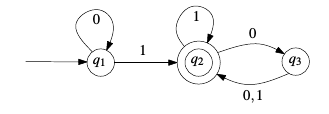
\includegraphics[scale=0.5]{images/states}
	\caption{A state diagram}
	\label{fig: state diagram}
\end{figure}
\begin{itemize}
	\item 	Design a DFA\footnote{Deterministic finite automata} for a problem ?
	\item 	How do we specify a problem ?
	\item 	To determine if the number of men is even or odd
\end{itemize}
To specify a problem is to specify a set of stings we would like to accept or not. 

\subsection{Deterministic Finite Automata}
\begin{figure}
	\centering
	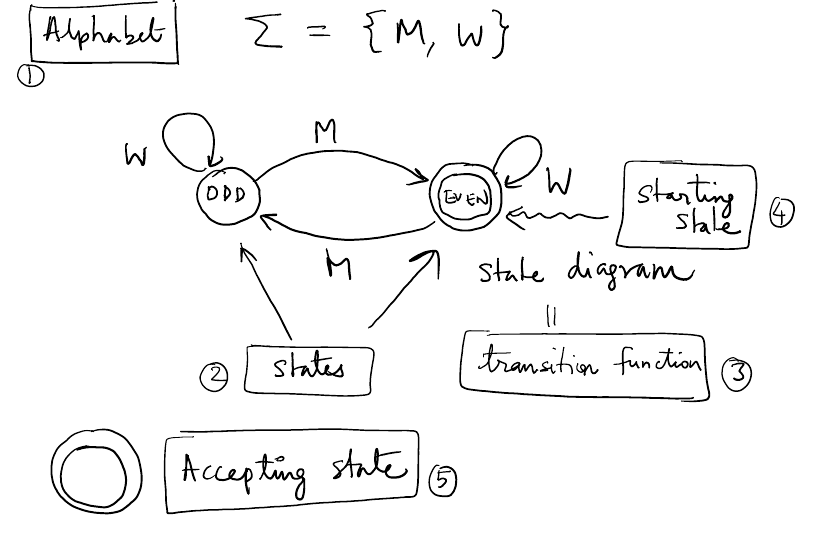
\includegraphics[scale=0.5]{images/DFA}
	\caption{The essential part of a DFA}
	\label{fig: dfa}
\end{figure}
\begin{boite}
	\evid{Notation :}
	\begin{enumerate}
		\item 	$\Sigma$ the alphabet (for example, $\Sigma = \{0,1\}$)
		\item 	$\Sigma^*$ the set of all possible strings from $\Sigma$ (for the previous alphabet, it would be all possible binary strings)
		\item 	\uline{Language} accepted by a machine
		\item 	$M$ denotes the DFA
		\item 	$L(M) = \{ \omega \in \Sigma^* : M$ accepts $\omega\}$ with property $L(M) \leq \Sigma^*$. It represents the ``problem we are trying to solve''.
	\end{enumerate}
\end{boite}
\begin{blackbox}

	\evid{Formal definition} : a deterministic finite automatin (DFA) $M$ is a 5-tuple ($Q, \Sigma, \delta, q_0, F)$ with :
	\begin{itemize}
		\item 	$Q$ - Set of states
		\item 	$\Sigma$ - Alphabet
		\item 	$\delta : Q \times \Sigma \to Q$ - the transition function
		\item 	$q_0$ - start state
		\item 	$F \subseteq Q$ - set of accepting states (allow $F = \emptyset$).
	\end{itemize}
\end{blackbox}
\begin{boite}
	\centering
	$L$ is a \textbf{regular language} if there is a DFA $M$ such that $L = L(M)$
\end{boite}
Not all languages are necessarily regular. 
\begin{exemple}~
	\begin{itemize}
		\item	$L = \Sigma^*$ this is a regular language (represent an unique state, accepting and starting, with all input leading to itself)
		\item 	All binary strings which have ``00'' in them.
				Is $L(M) = L$ ? 
	\end{itemize}
\end{exemple}
\subsubsection*{New language from old}
\begin{itemize}
	\item 	Complement : $\overline{L} := \{\omega \in \Sigma^* : \omega$ is \textbf{not in} $L\}$
	\item 	Union : $L_1 \cup L_2 := \{\omega \in \Sigma^* : \omega \in L_1$ \textbf{or} $\omega \in L_2\}$
	\item 	Intersection $L_1 \cup L_2 := \{\omega \in \Sigma^* : \omega \in L_1$ \textbf{and} $\omega \in L_2\}$
	\item 	Concatenation : $L_1 \degre L_2 := \{\omega \in \Sigma^* : \omega = \omega_1 \degre \omega_2, \omega_1 \in L_1$ \textbf{and} $\omega_2 \in L_2\}$
\end{itemize}
\todo{understand proof on union...}
\subsection{Post-Summary}
\begin{figure}
	\centering
	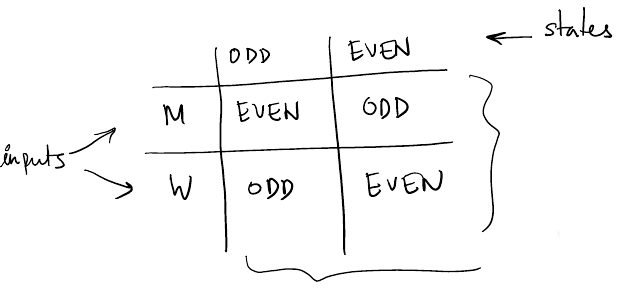
\includegraphics[scale=0.5]{images/table_state}
	\caption{Example of a table of inputs/states}
	\label{fig: table input/state}
\end{figure}
\begin{itemize}
	\item 	A DFA $M$ is a 5-tuple $M = (Q, \Sigma, \delta, q, F)$
	\item 	Q is the (finite) \textbf{set of all states }(like $q_1,q_1,q_3,...$)
	\item 	$\Sigma$ is the \textbf{alphabet} ; elements of it are \textbf{symbols} (for binary, we have $\Sigma = \{0,1\}$)
	\item 	$\Sigma^*$ is the set of all possible strings made out of combinations of the symbols of the declared $\Sigma$. For binary, it would be all possible binary strings (0, 1, 10, 11, 100, 101,...). Includes the empty string $\epsilon$
	\item 	$\delta : Q \times \Sigma \to Q$ is the \textbf{transition function}. It's represented with a table of inputs/states describing the next state (see figure \ref{fig: table input/state}) or a \textit{state-diagram} (see figure \ref{fig: state diagram})
	\item 	$q$, an element of $Q$, is the (unique) start state
	\item 	$F$ is a set (subset of Q) of all (but at least 1) accept states
	\item 	$L$ is the language ; $L(M)$ is the language of the DFA M, and represents all accepted strings ; with the example of odd/even number of men, if we place the accepting state on "odd" then the language is all the compositions of men and women such that we have an odd number of men.
	\item 	$A$ is a \textbf{regular} language if there exists a DFA $M$ such that $A = L(M)$
\end{itemize}



\section{Lecture 2 : Nondeterministic finite automaton}
A deterministic computation starts at a certain state and, at every symbol, change (or not) the state until the end of the string. At the end, your string is either accepted or rejected. 

A contrario, \textbf{nondeterministic computation} allows you to branch (one or multiple times), meaning at a given state, you can go to multiple states. This computation allows you to explore many possibilities at the same time. You have more possibilities with non-DFA : for example, you can now have 2 output from a state with same symbol (1 could lead you to 3 different states). Also, you can lack some symbols on a state (meaning you don't have to set a complete table, from a state you can set the 1 and not the 0). Finally, you can decide that from $q_i$ to $q_j$, you need a 0 or simply an empty string ($\epsilon$, so no symbol at all).

To determine if a string is accepted, we draw a tree of all possible states at every symbol. A string is accepted if, at the end, the last row has at least one accepting state.

Formally : 
\begin{boite}
    A \textbf{non deterministic finite automaton} (NFA) $N$ is a 5-tuple $(Q, \Sigma, \delta, q_0, F)$ with :
    \begin{itemize}
        \item     $Q$ : finite set of states
        \item     $\Sigma$ : finite alphabet
        \item     $\delta : Q \times \Sigma \cup \{\epsilon\} \to$ \textbf{Powerset($Q$)} - transition function
        \item     $q_0$ : start state
        \item     $F \subseteq Q$ : set of accepting states (allow$ F = \emptyset$)
    \end{itemize}
    $x$ is \textit{accepted} if there \textit{exists at least one path} that starts at a starting state and ends at an accept state (\textbf{Guess and verify !}).
    
    $x$ is \textit{rejected} if  \textit{no computation path} from any start state leads to an accept state.
\end{boite}
Language accepted by an NFA $N$ is the set of all words accepted by it : $L(N)$.

\subsection{Does every NFA have an DFA ?}
\begin{boite}
    \evid{Theorem :} For every NFA $N$, there exists a DFA $M$ s.t. $L(M) = L(N)$.
\end{boite}
\begin{itemize}
    \item     $N = (Q_N, \Sigma, \delta_N, q_0, F_N)$
    \item     $\hat{\delta}_N : 2^{Q_N} \times \Sigma^* \to 2^{Q_N}$\\
              $\hat{\delta}_N(A,\epsilon) = A$\\
              $\hat{\delta}_N(A,xa) = \bigcup_{q \in\delta_N(A,x)}\delta_N(q,a)$ \todo{accents !}
\end{itemize}
\begin{blackbox}[0.75]
\evid{Lemma :} for all $x,y \in \Sigma^* : \hat{\delta}_N(A,xy) = \hat{\delta}_N (\hat{\delta}_N(A,x),y)$\\
\uline{Proof :} induction on $|y|$ (exercise).
\end{blackbox}
\begin{itemize}
    \item     $M = (Q_M, \Sigma, \delta_M, q_0, F_M)$\\
              $Q_M = 2^{Q_N}$\\
              $F_M = \{A \subseteq Q_N : A \cap F_N \neq \emptyset\}$\\
              $\delta_M(A,a) = \hat{\delta}_N(A,a)$
\end{itemize}
\begin{blackbox}[0.73]
    \evid{Lemma :} For all $A \subseteq Q_N, x \in \Sigma^* : \hat{\delta}_M(A,x) = \hat{\delta}_N(A,x)$ \\
    \uline{Proof} : %TODO
\end{blackbox}
\todo{complete ?}
\evid{Proof of theorem :} \[x \in L(M) \iff \hat{\delta}_M(q_0, x) \in F_M \iff \hat{\delta}_N(q_0,x) \cap F_N \neq \emptyset \iff x \in L(N)\]
\subsubsection{Example}
\begin{figure}
    \begin{floatrow}
        \centering
        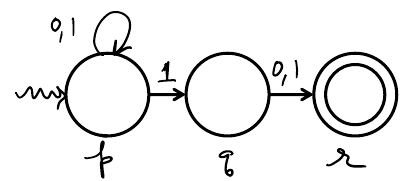
\includegraphics[scale=0.5]{images/nfa_dfa}
        \begin{tabular}{|c|c|c|}
            \hline
        	                & 0                & 1 \\
            \hline
            $\emptyset$     & $\emptyset$      & $\emptyset$ \\
            $\{p\}$         & $\{p\}$     	   & $\{p, q\}$\\ 
            $\{q\}$ 	& $\{r\}$  	   & $\{r\}$ \\
            $\{r\}$ 	& $\{\emptyset\}$  & $\{\emptyset\}$\\ 
            $\{p, q\}$ 	& $\{p, r\}$  	   & $\{p, q, r\}$\\ 
            $\{p, r\}$ 	& $\{p\}$  	   & $\{p, q\}$\\ 
            $\{q, r\}$ 	& $\{r\}$  	   & $\{r\}$ \\
            $\{p, q, r\}$ 	& $\{p, r\}$  	   & $\{p, q, r\}$ \\
            \hline
        \end{tabular}
    \end{floatrow}
    \caption{A NFA and its complete transition table}
    \label{fig: nfa to dfa}
\end{figure}
How to find the corresponding DFA of the graph at figure \ref{fig: nfa to dfa} (left)?  
\begin{enumerate}
    \item Fill a table ; lines correspond to the powerset of states $(p,q,r)$ will lead to $2^3$ lines : $\{\emptyset\}, \{p\}, \{q\}, \{r\}, \{p,q\}, \{p,r\}, \{q,r\}, \{p,q,r\}$.
    \item Then, for each of ``new states'', calculate the next state. A given next state is the union (no double) of all next states. For example, the next state of $\{p,q\}$ with 1 is the union of $\{p,q\}$ (possible next states of $p$ after 1) and $r$ (only next state of $q$ after a 1). This gives us $\{p,q,r\}$. We end up with figure \ref{fig: nfa to dfa} (right),
    \item Finally, go from starting state (here $p$) and retain all reachable states. Clearly, state $q$ is not reachable, so we don't pick it. Only states $\{p\}, \{p,q\}, \{p,r\}$ and $\{p,r,q\}$ are reachable. 
    \item Now just draw those states, and simplify your transition table with only these states. Tadaa !
\end{enumerate}

\subsection{Closure properties}
\begin{figure}
    \centering
    \begin{subfigure}{0.45\textwidth}
        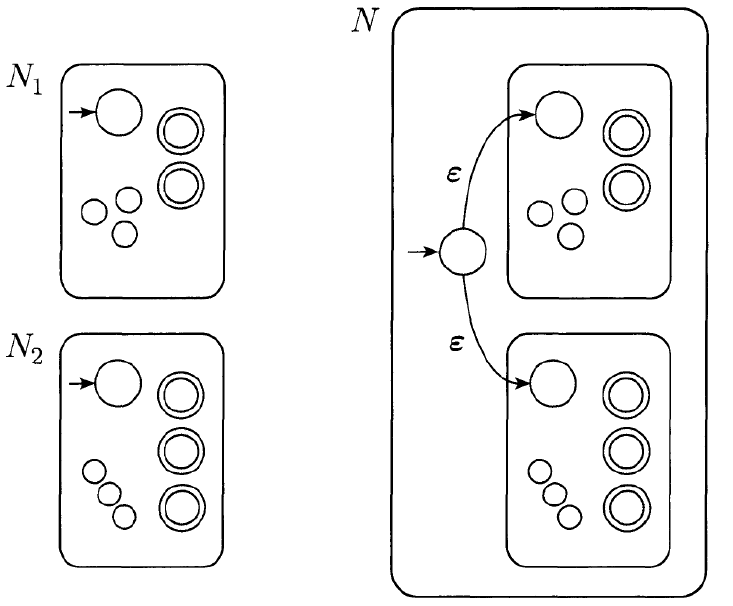
\includegraphics[scale=0.3]{images/union}
        \caption{Union}
        \label{subfig: union DFA}
    \end{subfigure}
    \begin{subfigure}{0.45\textwidth}
        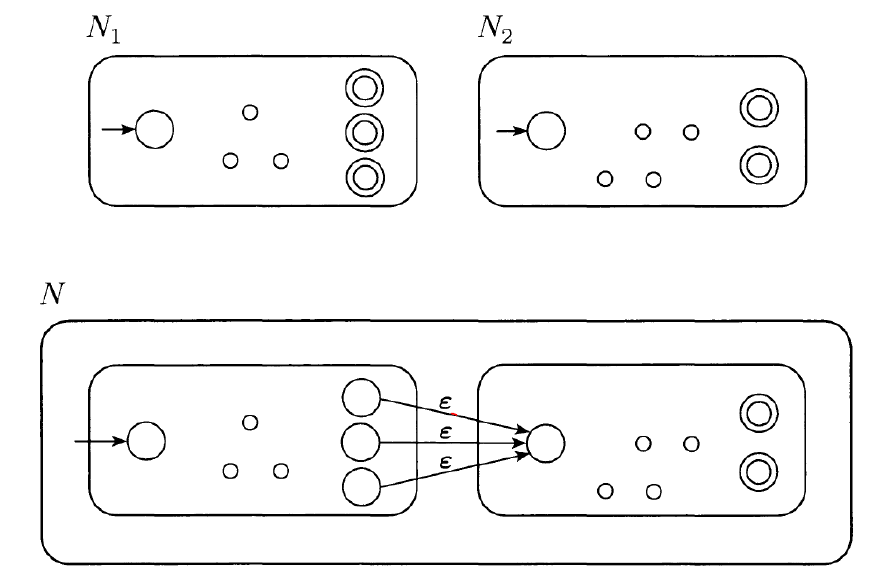
\includegraphics[scale=0.3]{images/concatenation}
        \caption{Concatenation}
        \label{subfig: concat DFA}
    \end{subfigure}
    \begin{subfigure}{0.45\textwidth}
        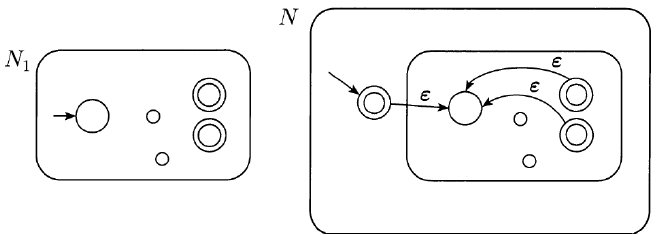
\includegraphics[scale=0.5]{images/kleene_dfa}
        \caption{Kleene enclosure}
        \label{subfig: kleene dfa}
\end{subfigure}
    \caption{Operations with two DFAs}
\end{figure}
We can combine multiple DFAs to obtain a ``larger one''. We can take the union, so all strings accepted by one or the other ; this is obtained by creating a new starting state, and from it requesting $\epsilon$ to go to both former starting states. Illustrated at figure \ref{subfig: union DFA}.

Also, we can do  the concatenation : all accepted strings are decomposable in 2 parts : the first is an accepted string of the first DFA, and second is an accepted string of the second DFA. Visible at figure \ref{subfig: concat DFA}.

Finally, we can do the Kleene enclosure. This is similar to writing $\Sigma^*$, it represents all possible combinations of the machine. Sub-strings of the accepted strings are also accepted strings. To be seen at figure \ref{subfig: kleene dfa}
\subsection{Post-Lecture Summary}
\begin{itemize}
    \item     A \textbf{non}-deterministic finite automaton (NFA) is a 5-tuple $(Q, \Sigma, \delta, q_0, F)$ with :        \begin{itemize}
                  \item $Q$ - a finite set of states
                  \item $\Sigma$ - the finite alphabet
                  \item $\delta: Q \times \{\Sigma$\textcolor{red}{$\cup \{\epsilon\}$}$\} \to$ \textcolor{red}{Powerset}($Q$) - the transition function
                  \item $q_0$ the (unique) start state
                  \item $F \subseteq Q$ - set of accepting states (allow $F = \emptyset$)
              \end{itemize}
              A very important difference with the DFA is that DFA needed to have all transition defined (every state had to know how to react with all symbols). Now, the NFA can have multiple next states with one symbol, and no transition for other symbols.
    \item     $x$ is \textbf{accepted} if there exists at least one path that starts at a starting state and ends at an accept state.
    \item     $x$ is \textbf{rejected} if \textbf{no computation path} from any start state leads to an accept state
    \item     We can always make  DFA from a NFA
\end{itemize}
\section{Lecture 3 : Non-Regular languages}
\subsection{What DFAs/FNAs can do :}
\begin{enumerate}
    \item     Pattern matching
    \item     Check divisibility by a fixed number
\end{enumerate}
Some languages are regular, some other are not. For example, here is a non-regular language :
\[B = \{0^n1^n: n \geq 0\}\]
Assume B is regular and let $M = \{Q, \Sigma, \delta, q_0, F\}$  be a DFA s.t. $L(M) = B$. The, let $|Q| = p$, pick $n \geq p$. Let $q_0$ be a start state and let $r = \hat{\delta}(q_0, 0^n1^n)$. Recall $\hat{\delta}(q_0, w)$ tells us the state after reading the entire word $w$. Now :
\[q_0 = s_1 \overset{0}{\to} s_2 \overset{0}{\to} s_3 \overset{0}{\to}... \overset{0}{\to} s_n \overset{0}{\to}s_{n+1} \overset{1}{\to} s_{n+1} \overset{1}{\to} s_{n+2} \overset{1}{\to} ... \overset{1}{\to} s_{2n} \overset{1}{\to} s_{2n+1} = r \in F\]
Because $n$ is bigger than $p$, two states have to repeat among $s_1,...,s_{n+1}$ ! Say $s_i = s_j = q \in Q$ and $1 \leq i \leq j \leq n+1$ $\to \hat{\delta}(q, 0^{j-i} = q$ Hence, $r = \hat{\delta}(q_0, 0^n1^n) = \hat{\delta}(q_0,0^i0^{j-i}0^{n-j}1^n) = \hat{\delta}(q_0,0^i0^{n-j}1^n)$. As $(h-j+i) \neq n \to M$ only accepts strings outside of $B$. That's a contradiction, proving that the language is not regular.

\evid{Other Example} :
\[C = \{w|w \text{ has an equal number of 0s and 1s}\}\]
Take previous example.

\evid{Pumping Lemma :} if $A$ is a ragular language, then there is a number $p$ (the pumping length) where, if $s$ is any string i A of length at least $p$, then $s$ may be divided into three pieces, $s = xyz$ satisfying the following conditions :
\begin{itemize}
    \item     For each $i \geq 0$, $xy'z \in A$
    \item     \todo{compléter}
\end{itemize}
\section{Lecture 4 : Turing machines}
\subsection{Quick recap}
Lecture 1 : DFA and regular languages. Lecture 2 : NFA and its equivalence to DFA. Lecture 3 : Non-regular languages and the Pumping lemma.
\begin{itemize}
    \item     $B = \{0^n1^n: n \geq 0\}$ cannot be recognized by DFAs
    \item     But... this seems like a problem with DFAs
    \item     What's missing ? We lack 
\end{itemize}
\subsection{Turing machines}
We often lack memory with DFAs. We can't remember a state, or if we already passed it once. We then define the basic of a Turing machine : 
\begin{center}
    DFA + Memory = Turing machine
\end{center}
You are given an infinite tape, with infinite number of cells. You have a small head, that treats one cell at a time. Head can \textbf{Read/write/move} left or right. Depending on what it does at a given cell, the head might change its state. Among all the possible states, it has accept but also \textbf{Reject} states. The tape's alphabet \uline{contains} input alphabet but might also have its own symbols that the head is not allowed to use. For example, it's probable that the tape contains some \textbf{blank symbols}. It may never reach an accept or reject state, and it might never halt ! That's new !\\
\evid{Differences between DFA and TM}
\begin{itemize}
    \item     A turing machine can both write on the tape ???
    \item     \todo{compléter}
\end{itemize}
\evid{Formal definition}
A \textbf{Turing machine} is a 7-tuple $(Q, \Sigma, \Gamma, \delta, q_0, q_{accept},q_{reject})$ where $Q,\Sigma, \Gamma$ are all finite sets and :
\begin{enumerate}
    \item $Q$ is the set of states
    \item $\Sigma$ is the input alphabet, not containing the blank symbol $\underbracket{\quad}$
    \item $\Gamma$ is the tape alphabet, where $\underbracket{\quad} \in \Gamma$ and $\Sigma \subseteq \Gamma$
    \item $\delta : Q \times \Gamma \to Q \times \Gamma \times \{L,R\}$ is the transition function
    \item $q_0 \in Q$ is the start state
    \item     $q_{accept}$ is the accept state
    \item     $Q_{reject}$ is the reject state, where $q_{reject} \neq q_{accept}$ 
\end{enumerate}
\evid{Configuration of a TM} : we describe 3 symbols : u left of actual state, v right of state (including actual position) and q, your actual symbol (at your actual position). We concatenate $uqv$ with $u,v \in \Gamma^*$ and $q \in Q$. All cells whose content is not specified are blank. If $u = \epsilon$, the the head is at the leftmost transition.

\evid{Transitions} Given $uqv,\ v = az$ for some $a \in \Gamma$ and $z \in \Gamma^*$ :
\begin{itemize}
    \item $u$\textcolor{red}{$a'$}$q'z$ if $\delta(q,a) = (q',a',R)$
    \item $u'q'$\textcolor{red}{$ba'$}$z$ if $u = u'b$ and $\delta(q,a) = (q',a',$\textcolor{red}{$L$})
    \item $uq'a'z$ if $u = \epsilon$ and $(q,a) = (q',a',L)$
    \item At any moment, you might be at position $u^1q_1v^1,\ u^2q_2v^2...u^tq_tv^t$
    \item The beginning must look like $q_0w$
    \item Accept state $u^t q_{accept} v^t$
    \item Reject state : $u^t q_{reject} v^t$
    \item Transition : $u^t q_t v^t \to u^{t+1} q_{t+1} v^{t+1}$
\end{itemize}
\subsection{Example}
Let 
\[C = \{w | w \text{ has an equal number of 0s and 1s}\}\]
Easy (efficient) to write an algorithm to counting number of 1s and 0s --- cumbersome to implement on a TM. In this Part(2) of the course, we do not care about running time. Our approach : check that for each 0 (or 1) there is a corresponding 1 (or 0).
\begin{enumerate}
    \item Scan the input from left to right
    \item Whenever we encounter an uncrossed 0 or 1, we cross it and proceed right to find a corresponding 1 or 0.
    \item We keep doing this (2) until either we cross off all the letters (accept) state or we fail to find a pair for one of the crossed letters (reject)
\end{enumerate}
\subsection{More}
\evid{Recognizable/Decidable languages :}\\
$M$ \textbf{accepts} $w \in \Sigma^*$ if $\exists C_1,C_2,...,C_t$ s.t. : $C_1$ is the starting state configuration of $M$ on $w$ ; $C_i \to C_{i+1}$ is one step of the TM $\forall i$ ; $C_t$ is an accepting configuration.
\[L(M) = \{w: M \text{ accepts }w\}\]
TM $M$ \textbf{recognizes} a language $L \subseteq \Sigma^*$ iff for all inputs $w \in \Sigma^*$ :
\begin{enumerate}
    \item If $w\in L$ then $M$ accepts $w$ and
    \item If $w \notin L$ then $M$ either rejects or never halts
\end{enumerate}
TM $M$ \textbf{decides} a language $L \subseteq \Sigma^*$ if for all inputs $w \in \Sigma^*$ :
\begin{enumerate}
    \item $M$ halts on $w$
    \item $M$ accepts w iff $w \in L$
\end{enumerate}
The natural questions at this point are : Is every language decidable ? Is every language recognizable ?
\subsection{Variants of TM}
\evid{Multitape TM} 
\[\delta : \Q \times \Gamma^k \to Q \times \Gamma^* \times \{L,R,S\}^k\]
Where $k$ is the number of tapes. The expression
\[\delta(q_i,a_1,...,a_k) = (q_j,b_1,...,b_k,L,R,...,L)\]
\begin{boite}
    \evid{Theorem 3.13} Every multitape Turing machine has an equivalent single tape Turing machine.
\end{boite}
S = ``On input $w = w_1\ldots w_n$ : 
\begin{enumerate}
    \item First, S puts its tape into the format that represents all $k$ tapes of M. The formatted tape contains 
    \todo{drôle de dessins...}
    \item To simulate a single move, S scans its tape from the first \#, which marks the left hand end, to the (k+1)st \#, which marks the right-hand end, in order to determine the symbole under the virtual heads. \todo{complete}
\end{enumerate}
\evid{Non-deterministic TM :} 
\[\delta : Q \to \Gamma \to P(Q\times \Gamma \times \{L,R\})\]
\begin{boite}
    \evid{Theorem 3.16 :} every non-deterministic Turing machine has an equivalent deterministic Turing machine (proof : in the book)
\end{boite}
\section{Lecture 5 : determinism and non-determinism}
\subsection{Recap}
We have an infinite tape, and a head that moves left/right and can read and write. The head has states. When reading a symbol on the tape, it moves and/or write and changes (or not) its state. The tape alphabet contains input alphabet and \textcolor{red}{blank symbols}. We can read blank symbols but the head \textbf{cannot write blanks}. The difference is that they may never reach an accept/reject state : they may never halt !

\evid{Configuration of a TM :} states strictly before where your head is $(u)$, and states after (and your current place) $v$. At your current state, the head is at state $q$. We then have a string $uqv$, where $u,v \in \Gamma^*$ and $q \in Q$. All cells whose content is not specified are blank. 
\begin{exemple}
    If we have the string $101101111...$ and are at second 0 with state $q_7$, we write 
    \[1011q_701111\]
\end{exemple}
\todo{petit trou ?}

\evid{REcognizable/decidable languages :} $M$ \textcolor{red}{accepts} $w \in \Sigma^*$ if $\exists C_1,C_2,...,C_t$ such that 
\begin{itemize}
    \item $C_1$ is the starting configutration of $M$ on $w$
    \item $C_i \to C_{i+1}$ is one step of the TM $\forall i$
    \item $C_t$ is an accepting configuration.
\end{itemize}
\[L(M) = \{w : M \text{ accepts } w\}\]

TM \textcolor{red}{recognizes} a language $L \subseteq \Sigma^*$ iff for all inputs $w\in \Sigma^*$
\begin{itemize}
    \item ig $w \in L$ then M accepts w and
    \item if $w \notin L$ then $M$ \textbf{either rejects w of never halts} 
\end{itemize}
L is recognizable is there is a TM that recognizes it

TM $M$ \textcolor{red}{decides} a language $L \subseteq \Sigma^*$ iff for all inputs $w \in \Sigma^*$ 
\begin{itemize}
    \item M halts on w
    \item M accepts w iff $w \in L$
\end{itemize}
\todo{manque une phrase}

\subsection{Simulating DFAs by a TM}
Let 
\[A_{DFA} := \Big\{\big< D, w\big> | D \text{ accepts } w \Big\}\]
\begin{itemize}
    \item $\big< B \big>$ - some canonical encoding of objects $B$ over binary alphabet
    \item All our TMs always preprocess to check validity of the input encoding and reject if it is not valid
\end{itemize}
Given $<D,w>$ :
\begin{enumerate}
    \item Simulate $D$ on $w$.
    \item Accept iff $D$ finishes reading $w$ in an accepting state.
\end{enumerate}

\subsection{Checking emptiness}
\[E_{DFA} := \big\{<D> | L(D) = \emptyset \big\}\]
Language accepted by a DFA is non-empty if and only if there is an accepting state that can be reached from the starting state by a sequence of transitions !

Given $<D>$, with $D = (Q,\Sigma, \delta, s, F)$ :
\begin{enumerate}
    \item Initialize $R := \{s\}$
    \item For each $q \in R...$
    \todo{compléter}
\end{enumerate}

\subsection{Two DFAs recognize the same language ?}
\[EQ_{DFA} = \big\{ <D, D'> | L(D) = L(D')\big\}\]
We could build symmetric difference : we have that $A \bigoplus B = (A \setminus B) \cup (B \setminus A)$. So :
\[L(D) \bigoplus L(D') = \overline{(L(D) \cap L(D')) \cup (\overline{L(D)} \cap \overline{L(D')}}\]
\todo{encore un trou...}

\subsection{The halting problem}
GIven a program, check if it works as specified.
\[A_{TM} = \Big\{\big< M, w\big> | M \text{ is a TM and } M \text{ accepts } w\big\}\]
$A_{TM}$ is recognizable
$U =$ ``On input, $<M,W>$, where M is a TM and $w$ is a string : 
\begin{enumerate}
    \item Simulate M in input w
    \item If $M$ ever enters its accept state, accept. If m ever enters is reject state, reject.''
\end{enumerate}
\begin{center}
    Is $A_{TM}$ decidable ?
\end{center}
Difficulty : conclude in finite numbers of steps that a given simulation of a TM $M$ on input $w$ will loop forever or not...

\subsection{$A_{TM}$ is undecidable}
Assume $H$ is a decider for $A_{TM}$.
\[H\big(<M,w>\big) = \left\{\begin{array}{ll}
    accept & \text{if M accepts } w\\
    reject & \text{if M does not accept } w
\end{array}\right.\]
$D =$ ``On input $<M>$, where $M$ is a TM :
\begin{enumerate}
    \item Run $H$ on input $\big<M, <M>\big>$
    \item output the opposite of what $H$ outputs; that is, if $H$ accepts, \textit{reject}, and if $H$ rejects, \textit{accept}''
\end{enumerate}
\[D\big(<M,w>\big) = \left\{\begin{array}{ll}
    accept & \text{if M does not accept } <M>\\
    reject & \text{if M accepts } <M>  
\end{array}\right.\]

\subsection{Unrecognisable languages ?}
\begin{boite}
    \evid{Theorem :} A language $L$ is decidable iff it is recognizable and its complement is also recognizable.
\end{boite}
\paragraph{Easy direction :} if $L$ is decidable, $L,\overline{L}$ are recognizable.

Assume $L, \overline{L}$ are recognizable
\begin{itemize}
    \item Let $M_1, M_2$ be the corresponding recognizers
            \begin{center}
                M = ``On input $w$ :
                \begin{enumerate}
                    \item Run both $M_1$ and $M_2$ on input $w$ in parallel.
                    \item If $M_1$ accepts, \textit{accept}; if $M_2$ a
\end{enumerate}
\end{center}
\end{itemize}
\todo{--'}
\section{Lecture 6 : Reducibility and reductions}
\subsection{Recap}
We know that 
\[A_{TM} = \{<M,w> |  ???\}\]
Given a language L, we want to know : is it recognizable ? decidable ? unrecognizable ?
\subsection{Reducibility}
\begin{boite}
    \evid{Reducibility :} Use knowledge about complexity of one language to reason about the complexity of other in an \textcolor{red}{easy} way.
\end{boite}
\begin{boite}
    \evid{Reduction :} Way to show that to solve one problem (A), it is sufficient to solve another problem (B). We write : \textcolor{red}{A reduces to B...}
\end{boite}
\begin{itemize}
    \item Many examples in real life. To know the area of a square, we can reduce the problem to finding a length.
    \item Reductions quantify \textcolor{red}{relative} hardness of problems. \textbf{If problem B is \textcolor{red}{easy}, then problem A is \textcolor{red}{easy} too}. But, \textbf{if problem A is \textcolor{red}{hard}, then problem B is \textcolor{red}{hard} too.}
\end{itemize}

\subsubsection{The case of \halt}
\[HALT_{TM} = \{<M,w> | M\text{ is a TM and M halts on input }w\}\]
\begin{boite}[0.6]
    \centering
    \evid{Theorem :} $HALT_{TM}$ is undecidable.
\end{boite}
A proof by contradiction :
\begin{itemize}
    \item Assume on the contrary that \halt is decidable.
    \item Let $R$ be a decider for it.
    \item Use R to construct a decider S for $A_{TM}$
\end{itemize}
$S = $``On input $<M,w>$, an encoding of a TM M and a string $w$ :
\begin{enumerate}
    \item Run TM $R$ on input $<M,w>$.
    \item If $R$ rejects, \textit{reject}
    \item If $R$ accepts, simulate $M$ on $w$ until it halts.
    \item If $M$ has accepted, \uline{accept}; if M has rejected, \textit{reject}''.
\end{enumerate}
\begin{itemize}
    \item Since $R$ rejects if and only if $M$ does not halt on $w$, $S$ is correct.
\end{itemize}

\subsubsection{The case of \reg}
\[\reg := \{<M> | TM\ M \text{ such that } L(M) \text{ is regular}\}\] 
\begin{boite}[0.6]
    \centering
    \evid{Theorem :} \reg is undecidable
\end{boite}
\begin{itemize}
    \item Assume on the contrary that \reg is decidable
    \item Le $R$ be a decider for it.
    \item Use $R$ to construct a decider $S$ for \atm
    \item $S$ takes input $<M,w>$ and modify $M$ such that resulting machine --$M_2$-- recognizes a regular language iff $M$ accepts $w$   
    \item \textbf{Design $M_2$ such that it always accepts a non-regular language ad accepts all the remaining strings from $\{0,1\}^*$ iff $M$ accepts $w$}
\end{itemize}
e$S =$ ``On input $<M,w>$, where M is a TM and w is a string :
\begin{enumerate}
    \item Construct the following TM $M_2$ : $M_2 =$ ``On input $x$ :
            \begin{enumerate}
                \item If $x$ has the form $0^n1^n$ \textit{accept}
                \item If $x$ does not have this form, run $M$ on input $w$ and \textit{accept} if $M$ accepts $w$.
            \end{enumerate}        
    \item Run $R$ on input $<M_2>$.
    \item If $R$ accepts, \textit{accept}; if $R$ rejects, \textit{reject}.
\end{enumerate}
\subsubsection{Reductions : Formally}
\begin{blackbox}
   \begin{itemize}
     \item A function $f: \Sigma^* \to \Sigma^*$ is a \textbf{computable function} if come Turing machine $M$, on every input $w$, halts with just $f(w)$ on its tape
     \item Language is \textbf{mapping reducible} to language $B$, written $A \leq_m B$, if there is a computable function $f: \Sigma^* \to \Sigma^*$, where for every $w$,
     \[w \in A \iff f(w) \in B\]
     The function $f$ is called the \textbf{reduction} of $A$ to $B$.
\end{itemize}
\end{blackbox}
\begin{boite}
    \evid{Theorem :} If $A \leq_m B$ and $B$ is decidable, then $A$ is decidable
\end{boite}
\begin{boite}
    \evid{Theorem :} 
    \[\atm \leq_m \halt\]
\end{boite}
\begin{itemize}
    \item Let us define a computable function $f$
    \item Given an input $x := <M,w>$, return $f(x) := <M',w>$ where
    \item $M' = $ ``On input $y$ :
            \begin{enumerate}
                \item Run $M$ on $y$
                \item If $M$ rejects $y$, enter an infinite loop. Otherwise, \textit{accept}
            \end{enumerate}
    \item $f$ is computable
    \item $\to$ if $<M,w> \in \atm$, then $M'$ halts on $w$. This, $<M',w> \in \halt$
    \item $\leftarrow$ if $<M,w> \notin \atm$, then either (1) will never halt or $M$ rejects $w$ and (2) will ensure no halting. Thus, $<M',w> \notin \halt$
\end{itemize}
\begin{boite}
    \evid{Theorem :}
    \[\atm \leq_m \reg\]
\end{boite}
\begin{itemize}
        \item Let us define a computable function $f$
        \item Fiuven an input $x := <M,w>$, return $f(x) := <M'>$ where
        \item $M' =$``On input $y$ :
                \begin{enumerate}
                    \item If $y \in B = \{0^n1^n\ : \ n \geq 0\}$ then \textit{accept}.
                    \item Run $M$ on $w$ and \textit{accept} if M accepts
                \end{enumerate}
        \item $f$ is computable
        \item $\to$ if $<M,w> \in \atm$, then $M'$ accepts all inputs. THus, $L(M') = \{0,1\}^*$ is regular --- $<M'> \in \reg$
        \item $\leftarrow$ If $<M,w> \notin \atm$, then $M$ does not accept $w$. Thus, $L(M') = B$ is non-regular --- $<M'> \notin \reg$
\end{itemize}
\subsection{Recognizable and co-unrecognizable}
\begin{boite}
    If $A \leq_m B$ and $B$ is recognizable, then $A$ is recognizable.
\end{boite}
\begin{itemize}
    \item Proof identical to the decidable case...
    \item \textbf{Corollary :} if $A \leq_m B$, and A is unrecognizable, then $B$ is unrecognizable.
\end{itemize}
We already know 
\[\eqtm = \{<M_1,M_2> | M_1 \text{ and } M_2 \text{ are TMs and } L(M_1) = L(M_2)\}\]
\begin{boite}
    \evid{Theorem :} \eqtm is unrecognizable and co-unrecognizable
\end{boite} 
\begin{itemize}
    \item We show $\overline{\atm} \leq_m \eqtm$
    \item Given an input $x := <M,w>$, return $f(x) := <M_1,M_2>$ where
    \item $M_1 =$ ``On input $y$ :
            \begin{enumerate}
                \item Run $M$ on $w$ (ignore the input $y$)
                \item If $M$ accepts the accept, else enter an infinite loop
            \end{enumerate}
    \item $M_2 =$ ``On input $y$ :
            \begin{enumerate}
                \item Reject $y$
            \end{enumerate}
    \item $f$ is computable
    \item $L(M_2) = \emptyset$ and
    \item $L(M_1) = \emptyset$ iff $M$ does not accept $w$.
    \item Thus, $<M,w> \in \overline{\atm}$ iff $<M_1,M_2> \in \eqtm$
    \item Similarly prove that $\overline{\atm} \leq_m \overline{\eqtm}$ (modify $M_2$ to accept all its inputs)
\end{itemize}
\section{Lecture 7}
\subsection{Recap}
We saw what is computable ? Decidable, undecidable, undecidable but recognizable, unrecognisable. Reductions. Undecidability=Hard, but decidability=easy
\subsection{Running time of a TM}
Let's take for example the machine 
\[B = \{0^k1^k : k \geq 0\}\]
With the machine :
$M =$ ``On input $w$ : 
\begin{enumerate}
    \item CHeck if $w \in \{0^*1^*\}$; if not, then reject
    \item Keep scanning $w$ from left to right, cross off an uncrossed $0-1$ pair each time
    \item Once either the last $0$ or the last 1 is crossed off, check if all the letters are crossed off; if YES, the \textit{accept}, else \textit{reject}.''
\end{enumerate}
\begin{center}
    \textbf{What is the running time of $M$ ?}
\end{center}
A problem with expectation is that we can't expect the same time for different input. One (bad) possibility is to describe the running time \uline{for each fucking possible input}. What is the time for $\epsilon$ ? $0$ ? 1 ? 10 ? 101101101 ? .... We need to understand how to \textbf{aggregate} all the informations for different inputs. Our best option is to consider always the \textcolor{red}{worst case}. We look for the input of length for which the machine is the worst. For a certain $k$, the length is $2^k$. We try to compute $t(k)$. Now a formal definition :
\begin{boite}
    \evid{Running time} \uline{Definition :} Let $M$ be a $TM$ that halts on all inputs (\textcolor{red}{decider}). The \textbf{\textcolor{red}{running time}} or \textbf{\textcolor{red}{time complexity}} of $M$ is the function $t: \N \to \N$ where 
    \begin{equation}
        t(n) = \max_{w \in \Sigma^* ; |w| = n} \text{number of steps M takes on }w
    \end{equation}
\end{boite}
So $M$ runs in time $t(n)$, with $n$ representing the length of the input.
\subsection{Big and small o}
\evid{Big-O} Let $f,g : \N \to \R_+$. We say $f(n) = O(g(n))$ if $\textcolor{red}{\exists C}\ \exists n_0$ s.t. $\forall n \geq n_0,\ f(n) \leq C\cdot g(n)$\\
\evid{Small-o} Let $f,g : \N \to \R_+$. We say $f(n) = o(g(n))$ if $\textcolor{red}{\forall c}\ \exists n_0$ s.t. $\forall n \geq n_0,\ f(n) \leq c\cdot g(n)$\\
\subsubsection{Example}
Let's take the same machine as before : $M =$ ``On input $w$ : 
\begin{enumerate}
    \item Check if $w \in \{0^*1^*\}$; if not, then reject
    \item Keep scanning $w$ from left to right, cross off an uncrossed $0-1$ pair each time
    \item Once either the last $0$ or the last 1 is crossed off, check if all the letters are crossed off; if YES, the \textit{accept}, else \textit{reject}.''
\end{enumerate}
Complexity :
\begin{enumerate}
    \item We just have to go through the list once : $O(n)$
    \item $O(n^2)$
    \item At the end, we start over to check if all are crossed. Pass the list once : $O(n)$
\end{enumerate}
\subsection{Time complexity}
\begin{boite}[1]
    \evid{Definition} Time complexity class :
    \begin{center}
        \textcolor{red}{$TIME\big(t(n)\big) := \{L \subseteq \Sigma^* | L$ is decided by a TM with running time $O\big(t(n)\big)\}$}
    \end{center}
\end{boite}
$--B \in TIME(n^2)$\\
But what about $TMs$ with multiple tapes ?
\begin{boite}
    \evid{Theorem} Let $t(n) \geq n$. Then every $t(n)$ time multiple tape $TM$ has an equivalent $O(t(n)^2)$ time single tape TM (proof in the book)
\end{boite}
\subsection{Non-deterministic TM}
Let $N$ be a $NTM$ that halts on all input (decider). The \textbf{running time} or \textbf{time complexity} of $N$ is the function $t: \N\to \N$ where
\begin{equation}
    \textcolor{red}{t(n) = \max_{w\in \Sigma^*; |w| = n} \text{ max \# steps $N$ takes on any computation branch ow $w$}}
\end{equation}

\subsection{P}
Which is more efficient ? $10000n^3$ or $(1.0001)^n$ ? With small inputs right is better, but with real life and Big Data, left is much more efficient.
\[TIME(n) \subseteq TIME(n^2) \subseteq \ldots \subseteq TIME(2^{\sqrt{n}}) \subseteq TIME(2^n) \subseteq TIME(2^{2^n})\]
\begin{boite}
     \evid{Definition 7.12 :} $P$ is the class of languages that are decidable in polynomial time on a deterministic single tape Turing machine. In other words : 
     \[P = \bigcup_k TIME(n^k)\]
\end{boite}
$P$ is invariant for all models of computation that are polynomially equivalent to deterministic single tape TM -- \textcolor{red}{robust}. $P$ also roughly corresponds to the class of problems that are realistically solvable -- \textcolor{red}{practical}
\subsubsection{P and Brute-force search}
\[PATH := \{\<G,s,t\> | \text{ there is an s-t path in G}\}\]
[see slides]
\section{Lecture 8 : NP, NP-Completeness}
\subsection{Recap}
\begin{blackbox}
    $P$ is the class of languages that are decidable in polynomial time on a deterministic single tape Turing machine. In other words :
    \[P = \bigcup_k TIME(n^k)\]
\end{blackbox}

\subsection{Hamiltonian path in a Graph}
A path from $s$ to $t$ that visits each node exactly once. We define a TM :
\[HAMPATH = \{\langle G,s,t\rangle | G \text{ is a directed graph with a Hamiltonian path from s to t}\}\]
\subsection{CLIQUE} 
A subset such that all vertices are connected with each others
\[CLIQUE = \{\langle G, k \rangle G \text{ is a undirected graph with a $k-$clique}\}\]
Here, the brute force implies testing all the subsets and testing if the given trial is a solution or not. 
\subsection{Polynomial Time verifiers}
If we have a solution and have to check whether or not this is a solution, that is easy.  In opposite, \uline{finding} a solution is hard. We want to formalize that difficulty.
\begin{blackbox}
    \evid{Definition 7.18} A \textbf{verifier} for a language $A$ is an algorithm $V$ where 
    \[A = \{w | V \text{ accepts } \langle w, c \rangle \text{ for some strings } c \}\]
    We measure the time of a verifier only in terms of the length of $w$, so a \textbf{polynomial time verifier} runs in polynomial time in the length of $w$. A language $A$ is \textbf{polynomially verifiable} if it has a polynomial time verifier.
\end{blackbox}
Both precedent problems have a polynomial time verifier. That's an easy job.

\subsection{NP}
\begin{blackbox}
    \evid{Definition 7.19 :} $NP$ is the class of languages that have polynomial time verifiers.
\end{blackbox}
$HAMPATH $ and $CLIQUE \in NP$. \textbf{Verifier :} $V_c$: On input $\langle\langle G,k\rangle C\rangle$
\begin{enumerate}
    \item Check if $C$ is a valid \todo{complete}
\end{enumerate}
\begin{blackbox}
    \evid{Theorem 7.20} A language is in $NP$ iff it is decided by some nondeterministic polynomial time Turing machine
\end{blackbox}
Let $N$ be a NTM that halts on all inputs (decider). The \textbf{running time} or \textbf{time complexity} of $N$ is the function $t : \N \to \N$ where 
\[t(n) = \max_{w \in \Sigma^*; |w| = n} \max \# \text{ steps N takes on any coimputation branch on $w$}\]
\begin{blackbox}
    Time complexity class :
    \[NTIME(t(n)) :=) \{L \subseteq \Sigma^* | L \text{is decided by a NTM with running time }O(t(n))\}\]
\end{blackbox}
\begin{boite}
    Theorem (restated) $NP = \bigcup_k NTIME(n^k)$
\end{boite}

\subsection{P vs. NP}
$P$ = the class of languages for which membership can be \textit{decided} quickly\\
$NP$ = the class of languages for which membership can be \textit{verified} quickly

Cook and Levin discovered that there is a problem in NP s.t. if you show it is in P, then $NP \subseteq P$. The satisfiability --- a.k.a. --- SAT

We use traditional boolean variables and logic. A formula :
\[\phi(x_1,x_2,x_3) = (\overline{x_1} \vee x_2) \wedge (x_1 \vee \overline{x_3})\]
A formula is \textbf{satisfiable} if there is an assignment to the variables which satisfies all the clauses.
\[SAT =  \{\langle \phi \rangle | \phi \text{ is a satisfiable Boolean formula}\}\]
By theorem : $SAT \in P \iff P = NP$. This is the starting point to establish hardness of other NP problems...
\subsection{Polynomial time reducibility}
\begin{blackbox}
    A function $f:\Sigma^* \to \Sigma^*$ is a \textbf{polynomial time computable function} if some polynomial time Turing machine M exists that halts with just $f(w)$ on its tape, when started on any input $w$.
\end{blackbox}
\begin{blackbox}
    Language A is \textbf{polynomial time mapping reducible} or simple \textbf{polynomial time reducible} to language $B$, written $A \leq_p B$ is a polynomial time computable function $f : \Sigma^* \to \Sigma^*$ exists where for every $w$ :
    \[w \in A \iff f(w) \in B\]
    The function $f$ is called the \textbf{polynomial time reduction} of A to B.
\end{blackbox}
Trivial theorem : If $A \leq_p Bb$ and $B \in P \to \overline{A} \in P$

\subsection{CLIQUE is NP-Complete}
Cook-Levin theorem : $SAT$ is NP-Complete and $3SAT$ is NP-Complete (when $2SAT \in P$)
\evid{Theorem :} $3SAT \leq_p CLIQUE$
\[\phi = \bigwedge^m_{j=1} \psi^j\]
$\phi^j$ is a disjunction of three literals $l_1^j,l_2^j,l_3^j$, i.e. $\psi^ j = l_1^j \vee l_2^j \vee l_3^j$

\section{Lecture 9 : more on NP-completeness}
\subsection{Reminder}
\begin{blackbox}
    $NP$ is the class of languages that have a polynomial time verifiers
\end{blackbox}
\begin{blackbox}
    
\end{blackbox}
\begin{blackbox}
    A function $f:\Sigma^* \to \Sigma^*$ is a \textbf{polynomial time computable function} if some polynomial time Turing machine M exists that halts with just $f(w)$ on its tape, when started on any input $w$.
\end{blackbox}
\begin{blackbox}
    Language A is \textbf{polynomial time mapping reducible} or simple \textbf{polynomial time reducible} to language $B$, written $A \leq_p B$ is a polynomial time computable function $f : \Sigma^* \to \Sigma^*$ exists where for every $w$ :
    \[w \in A \iff f(w) \in B\]
    The function $f$ is called the \textbf{polynomial time reduction} of A to B.
\end{blackbox}
\begin{boite}
    A language B is $NP-$complete if it satisfies two conditions :
    \begin{itemize}
        \item B is in NP
        \item every A in NP is polynomial time reducible to B
    \end{itemize}
\end{boite}

Trivial theorem :
\begin{enumerate}
    \item If B is NP-complete and $B \in P \to P = NP$
    \item If B is NP-complete and $B \leq_p C$ and $C \in NP \to C$ is NP-complete
\end{enumerate}
CLIQUE : A graph (set of edges and vertices) ; look for a subset such that all vertices are connected with every other.

\evid{Proof :} By Cook-Levin theorem : $3SAT$ is NP-Complete. By theorem : $3SAT \leq_p CLIQUE \to CLIQUE$ is NP-Complete 

Construct $\langle G, m\rangle$ as follow :
\begin{enumerate}
    \item G has a vertex $v_k^j$ for each literal in $\phi$
    \item G has an edge between two vertices $v_k^j$ and $v_s^i$ if and only if
            \begin{enumerate}[label=\alph*.]
                \item $j\neq i$
                \item The literal $l_k^j$ is not a negation of the literal $l_s^i$
            \end{enumerate}
    \item $m$ is the number of clauses in $\phi$
\end{enumerate}
e.g. : 
\[(\overline{x_1} \vee x_3 \vee x_5) \wedge (x_1 \vee \overline{x_3} \vee \overline{x_5}) \wedge (\overline{x_1} \vee \overline{x_3} \vee x_5)\]
\begin{enumerate}[label = STEP \Alph* :]
    \item Polynomial time reduction
    \item If $\phi$ is satisfiable $\to G$ has a clique of size $m$. No edge in a the triple, no exge connecting $x_i$ and $\overline{x_i}$.
    \item If $G$ has a clique of size $m \to \phi$ is satisfiable
\end{enumerate}

\subsection{Vertex cover}
Given $G = (V,E)$, find $C \subseteq V$ which ``covers'' all the edges. Edges are covered if : $\forall edge = i-j$ Must have either $i \in C$ or $j \in C$. Given a set of cities, for two villages, you must have a post office in one village or the other.
\[VERTEX-COVER = \{\langle G,k\rangle | G \text{ is an undirected graph that has a k-node vertex cover}\}\]
Vertex-Cover is NP-Complete
\begin{enumerate}[label=STEP \Alph*: ]
    \item Vertex Cover $\in NP$. TM V : On input $\langle\langle G,k\rangle c \rangle$ (with $c \subseteq V$)
    \begin{enumerate}
        \item Check if c is a valid encoding if a subset of vertices of G with of size $k$. Is no, \textit{reject}
        \item CHeck if c is a vertex cover. Is yes, \textit{accept}, 
    \end{enumerate}
\end{enumerate}

Given $3SAT$ formula $\langle \phi \rangle$ on n variables and m clauses. Construct $G$ as $f :$
\todo{?}

\listoftodos
\end{document}